\title{Assignment 2: Graph Visualization with GraphViz}
\author{
        %\large
        \textsc{Caitlin Ross}
  %          \qquad
     %   \textsc{}
        \mbox{}\\ %
        Department of Computer Science\\
        CSCI 6963\\
       %  \\
       % \mbox{}\\ %
        \normalsize
            \texttt{rossc3}
        \normalsize
            \texttt{@rpi.edu}
}
\date{\today}
\documentclass[11pt]{article}
%\documentclass{acmconf}

\usepackage[letterpaper,dvips,top=1.5cm,left=1.5cm,right=1.5cm,
    foot=1cm,bottom=1.5cm]{geometry}
%\usepackage[letterpaper, portrait, margin=2in]{geometry}
%\usepackage[a4paper,showframe=true,bindingoffset=0.2in,%
  %          left=1in,right=1in,top=1in,bottom=1in,%
   %         footskip=.25in]{geometry}

\usepackage{times}
%\usepackage{graphicx}
\usepackage[fleqn]{amsmath}
\usepackage{amsfonts}
\usepackage{amssymb}
\usepackage{amsthm}
\usepackage{amsopn}
\usepackage{xspace}
\usepackage{array}
\usepackage{epsfig}

\numberwithin{figure}{section}

\newcommand\CC{\Lang{\mbox{C++}}\xspace}
\newcommand\Lang[1]{\textsc{#1}}
\newcommand{\kw}[1]{\texttt{\textbf{#1}}}
\newcommand{\cd}[1]{\texttt{#1}}

\newcommand\Naturals{\ensuremath{\mathbb{N}}\xspace}
\newcommand\Integers{\ensuremath{\mathbb{Z}}\xspace}
\newcommand\Rationals{\ensuremath{\mathbb{Q}}\xspace}
\newcommand\Reals{\ensuremath{\mathbb{R}}\xspace}
\newcommand\Complex{\ensuremath{\mathbb{C}}\xspace}

\newcommand\norm[1]{\ensuremath{\lVert#1\rVert}}
\newcommand\abs[1]{\ensuremath{\lvert#1\rvert}}
\newcommand\ceil[1]{\ensuremath{\lceil#1\rceil}}
\newcommand\floor[1]{\ensuremath{\lfloor#1\rfloor}}
\newcommand\set[1]{\ensuremath{\{#1\}}}
\newcommand\angular[1]{\ensuremath{\langle#1\rangle}}

\newcommand\Norm[1]{\ensuremath{\left\lVert#1\right\rVert}}
\newcommand\Abs[1]{\ensuremath{\left\lvert#1\right\rvert}}
\newcommand\Ceil[1]{\ensuremath{\left\lceil#1\right\rceil}}
\newcommand\Floor[1]{\ensuremath{\left\lfloor#1\right\rfloor}}
\newcommand\Set[1]{\ensuremath{\left\{#1\right\}}}
\newcommand\Angular[1]{\ensuremath{\left\langle#1\right\rangle}}

\newcommand{\LOOM}{\ensuremath{\cal{LOOM}}\xspace}
\newcommand{\PolyTOIL}{\textbf{PolyTOIL}\xspace}

\newtheorem{theorem}{Theorem}[section]
\newtheorem{definition}[theorem]{Definition}
\newtheorem{lemma}[theorem]{Lemma}
\newtheorem{corollary}[theorem]{Corollary}
\newtheorem{fact}[theorem]{Fact}
\newtheorem{example}[theorem]{Example}

\newcommand\Cls[1]{\textsf{#1}}
\newcommand\Fig[1]{Figure~\ref{Figure:#1}}

\usepackage{labels} %
%\usepackage{equation}
%\usepackage{prog2tex}

\newenvironment{excerpt}{\begin{quote}\begin{minipage}\textwidth}{\end{minipage}\end{quote}}

\setcounter{topnumber}{0}
\setcounter{bottomnumber}{0}
\setcounter{totalnumber}{20}
\renewcommand{\textfraction}{0.01}

\begin{document}
\newgeometry{margin=1in}
\maketitle
\section{Introduction}
The purpose of this assignment is to use GraphViz and experiment with the different types of graphs and options available. I wrote a C program that uses GraphViz as a library and output the DOT files and PNG files for each graph (images are displayed in this document, while the DOT files are included in the zip file).  The program contains several options to choose which graph to create, as well as some basic parameters to change graphs.  Two of the graphs are either based on my own research project or data collected in class, while the other three graphs shown are just random examples of what can be done with GraphViz.  At the end of this writeup, I discuss my opinion on the GraphViz tool.  
\section{Graphs}
\begin{figure}[ht]
	\centering
		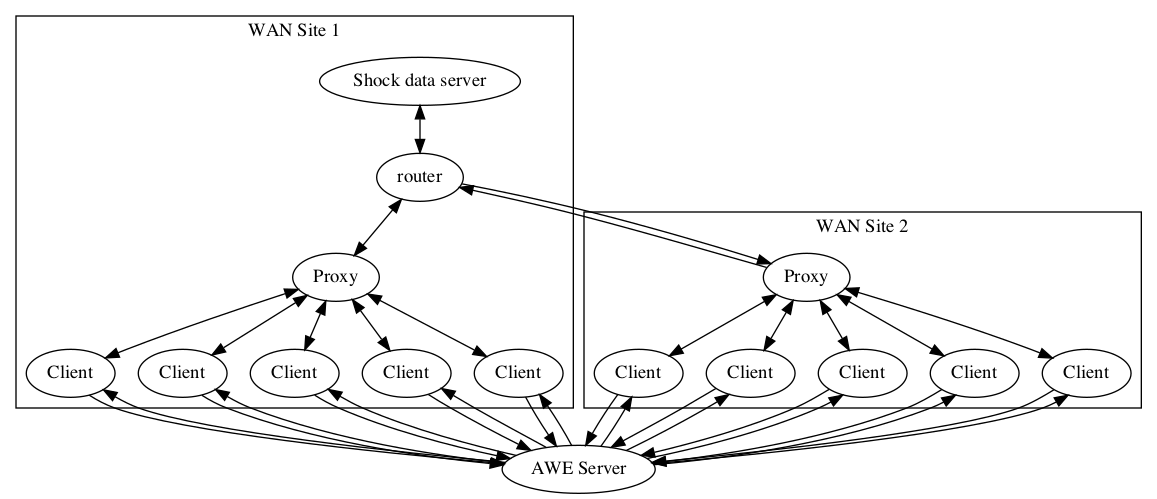
\includegraphics[width=6in]{awesim.png}
	\caption{MG-RAST infrastructure drawn with GraphViz}
	\label{fig:awesim}
\end{figure}
\begin{figure}[ht]
	\centering
		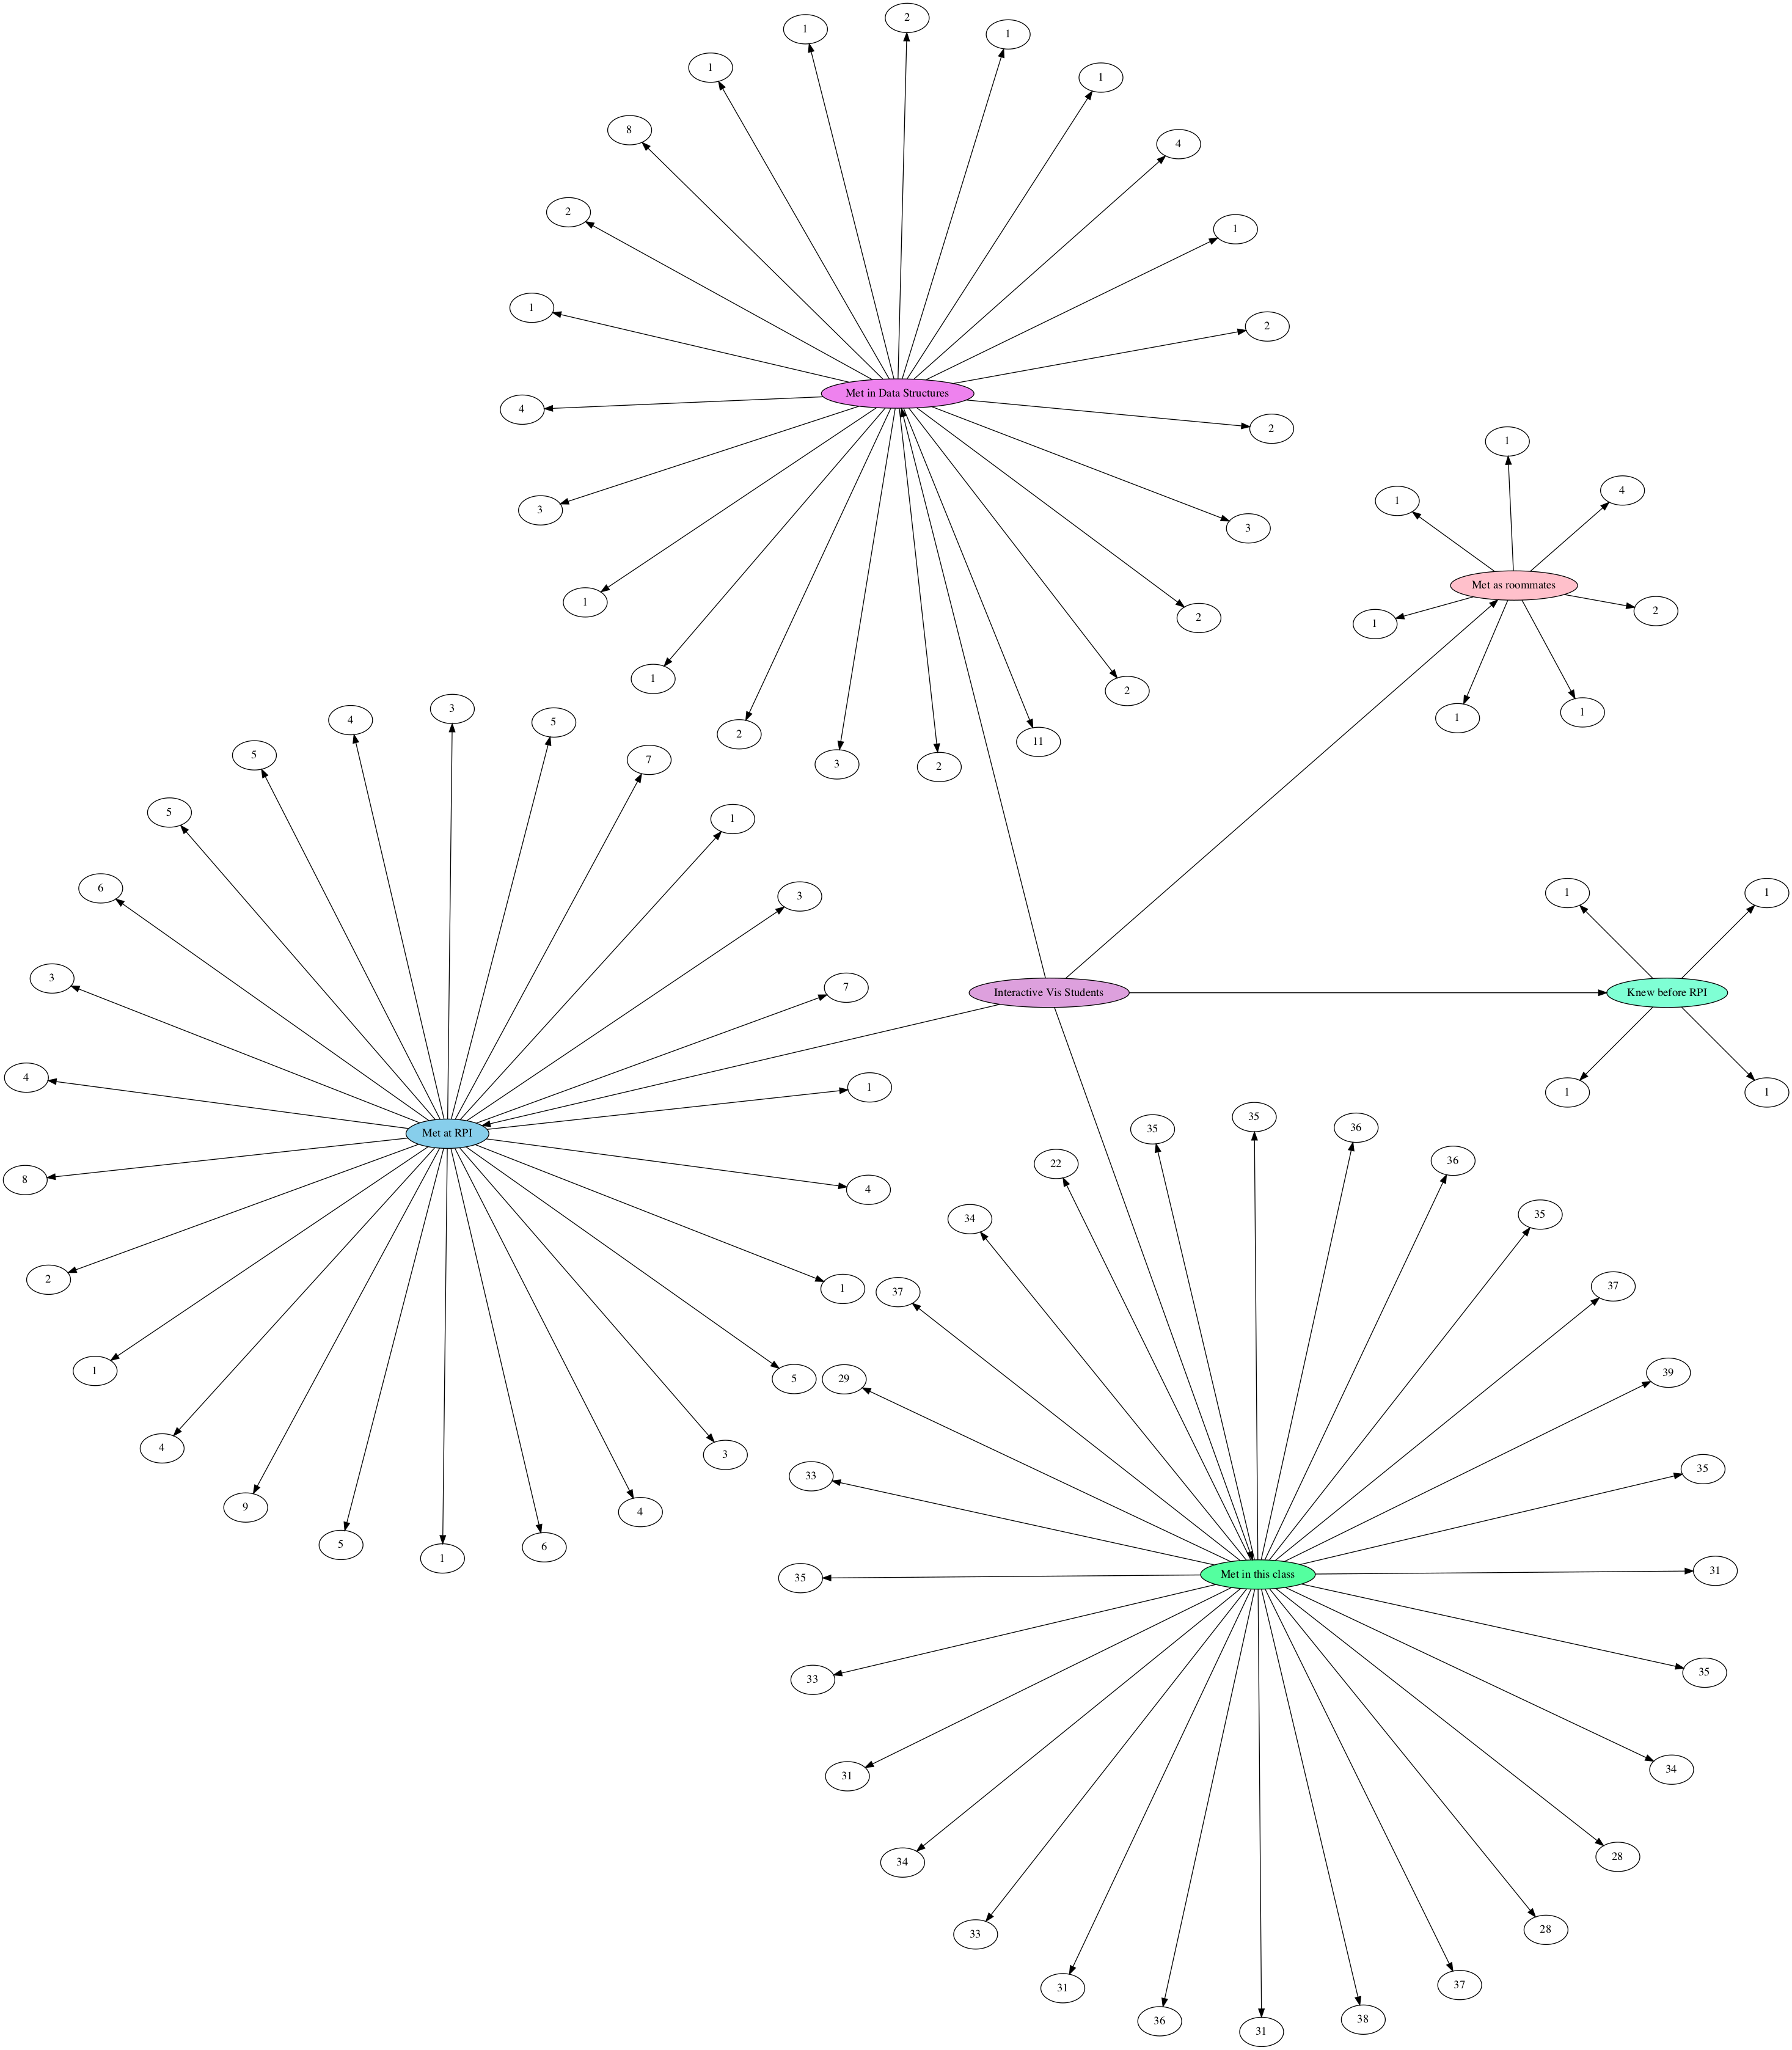
\includegraphics[width=6in]{class.png}
	\caption{Class data drawn with GraphViz}
	\label{fig:class}
\end{figure}
\begin{figure}[ht]
	\centering
		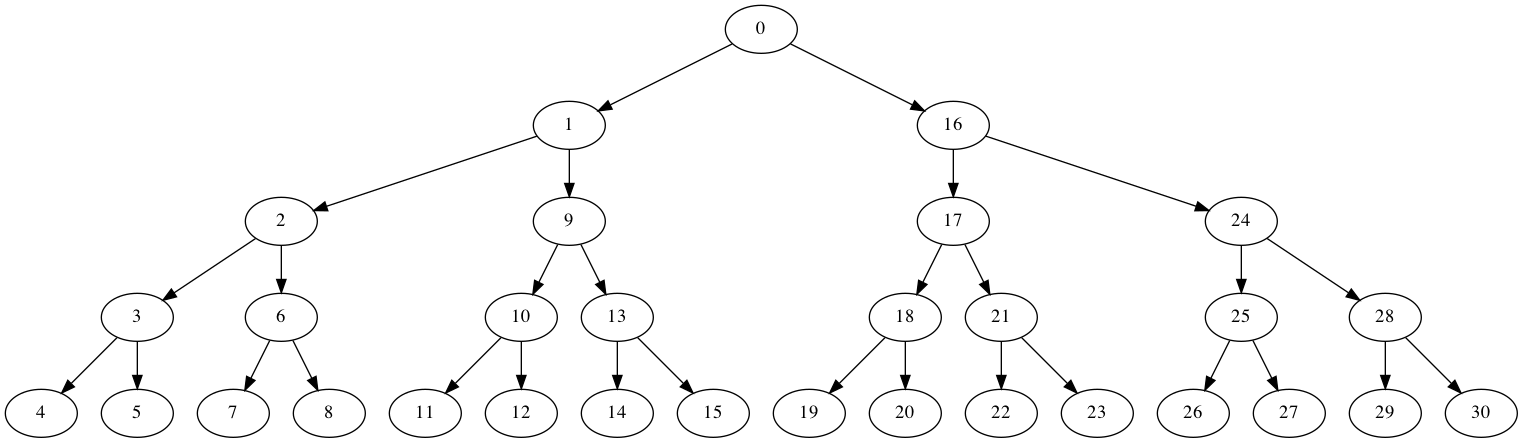
\includegraphics[width=6in]{tree.png}
	\caption{Tree with 5 levels created with GraphViz}
	\label{fig:tree}
\end{figure}
\begin{figure}[ht]
	\centering
		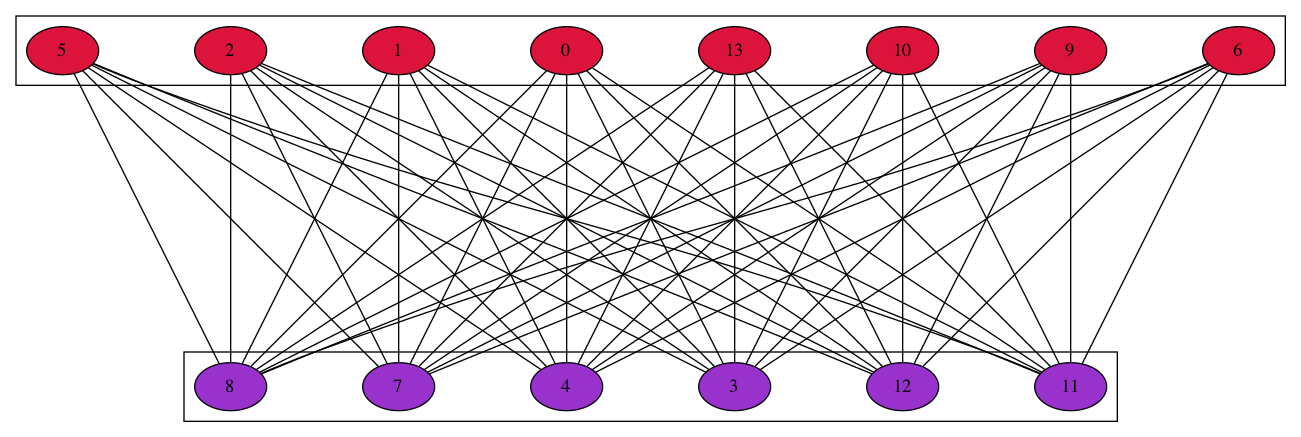
\includegraphics[width=6in]{bipartite.png}
	\caption{Bipartite graph with 14 nodes drawn with GraphViz}
	\label{fig:bipartite}
\end{figure}
\begin{figure}[ht]
	\centering
		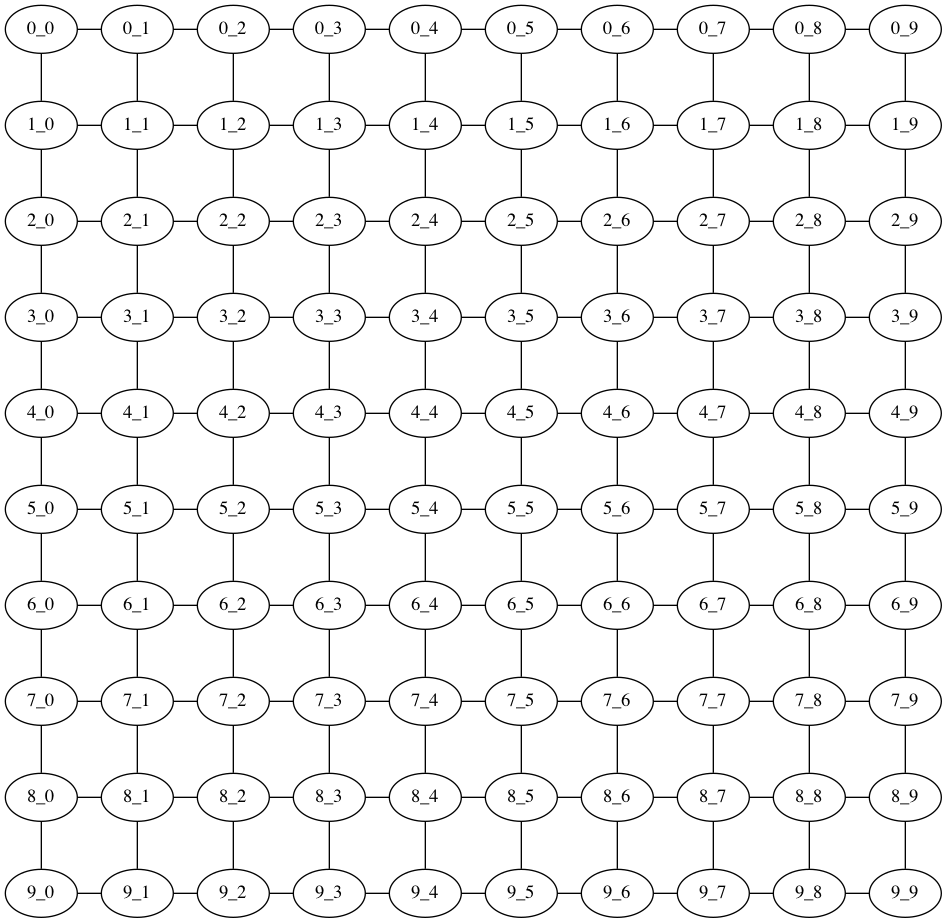
\includegraphics[width=6in]{square.png}
	\caption{$10 \times 10$ square drawn with GraphViz}
	\label{fig:square}
\end{figure}

Figure \ref{fig:awesim} is a graph based on my research.  I have been working on a simulation of a bioinformatics service called MG-RAST and this is what the infrastructure looks like.  There are two wide area network (WAN) sites in my simulation, each contains a storage proxy server for clients to contact, and the proxies connect to a centralized data server called Shock through a router. Then there is a scheduler, called the AWE Server, that schedules tasks among the clients.  The arrows represent the communication between entities in the system.  I was able to group each site together as a cluster.  Overall I think the layout turned out well, though it could use some more tweaking.  I tried to get all arrows to show as bidirectional, but for some reason that only worked within a cluster.  This graph can be created using my createdot program with the \texttt{--awesim} option.  Using \texttt{--nodes} allows the number of client nodes within each site to change.  Also, the \texttt{--undirected} option can be used to have undirected edges.  For papers, I've created diagrams of the MG-RAST infrastructure using Powerpoint and I think that is what I would continue to use for a diagram like this.  However, if I had a more complicated network to visualize, I would choose a tool like GraphViz.  

Figure \ref{fig:class} is a graph created based on the data we collected in class.  I have one root node that connects each of the 5 options we were given for when we met each person in class.  Each possible option shows each of the answers given in the table, unless the answer was 0.  For instance, 4 people met 1 other person before RPI, so there are 4 '1' nodes around the 'Knew before RPI' node.  My hypothesis before collecting data was that a lot of people had already met each other either in Data Structures or at RPI, but based on the graph, it appears most people didn't know each other before this Visualization class.  To put the graph in this circular format, I used the 'circo' layout.  I think for this particular dataset, this has a nice starburst look. To create the graph, the \texttt{--class-data} option with a path to the comma delimited file that contains the data to be used.

The next three graphs are not created from any particular dataset; they are just examples of various things that could be computed.  When selecting \texttt{--tree-levels=n}, where n is some integer, a binary tree with n levels is created.  Again, the \texttt{--undirected} option can be used here.  A tree with 5 levels is shown in Figure \ref{fig:tree}.  This was a really easy graph to create by recursion, so using the GraphViz library is probably a good tool to use if your data works well as a tree.

A bipartite graph is shown in Figure \ref{fig:bipartite}.  The creation of this graph used the options \texttt{--bipartite --undirected --nodes=14}.  The program randomly placed the nodes in one of the two clusters, then creates edges for each pair of nodes.  Here I played around with ranksep and nodesep settings which changes the sides between the ranks (or clusters) and nodes, respectively.  I also added some color fill into the nodes, with each cluster having it's own color.  

Finally, Figure \ref{fig:square} shows a $10 \times 10$ square with edges between immediate neighbors.  This graph used the options \texttt{--square --nodes=10 --undirected}.  I tried to actually create it as a torus, so that all nodes have 4 neighbors; however, I could never get that graph into a decent layout, no matter what settings I used.  I think this would be a graph that is probably better drawn manually, in order to choose the best placement of edges that wrap from one side to the other.  

\section{GraphViz Review}
I have two different machines that I work on, so I attempted to use GraphViz on both platforms: one is a Mac and the other runs Ubuntu.  Installation was very easy on both, but I had issues getting my code to run on my Ubuntu machine.  I think this is an Ubuntu issue and not a GraphViz issue.  

The basics of using GraphViz as a library was not too difficult.  The GraphViz website provides a library guide that was really helpful in learning how to use it. The guide also included tables of the various attributes that could be changed for graphs, edges, and nodes. The graphs I've created look simple and aren't too difficult to create, though I did spend a lot of time playing around with different settings. I think more complex graphs could be very difficult to find a decent layout with GraphViz and tweaking the settings would possibly take a really long time.  I also felt like some of the settings I used (e.g. bidirectional arrows) didn't work the way I thought they would, but I admit that this could be a user error.  I think in the future if I need a relatively simple graph, I will probably use GraphViz to create it since I am now familiar with it, but if I need to make a complex graph, I will probably look into other options.  
%\bibliography{main}

%\bibliographystyle{abbrv}
\end{document}
